\documentclass[11pt]{article}
\usepackage{fancyhdr}
\usepackage{graphicx}
\usepackage{amssymb,amsmath}
\usepackage{psfrag}
\usepackage{color}
\usepackage[colorlinks]{hyperref}
\usepackage[footnotesize,hang,bf]{caption}
\usepackage{subeqnarray}
% \usepackage{amsthm}
 \usepackage{enumitem}
 \graphicspath{{Figures/}}
 \usepackage{multicol}
 \usepackage{ marvosym }
 \usepackage{wasysym}
 \usepackage{tikz}
 \usetikzlibrary{patterns}

 \newcommand{\ds}{\displaystyle}
 \DeclareMathOperator{\sech}{sech}

%%%%%%%%%%%%%%%%%%%%%%%%%%%%%%%%%%%%%%%%%%%%%%%%%%%%%%%%%%%%%%%%%%%%%%%%%%%%%%%%%%

\def\hwnum{2}
\def\term{Spring 2018}

\setlength{\oddsidemargin}{0 in}
\setlength{\evensidemargin}{0 in}
\setlength{\topmargin}{0.0 in}
\setlength{\textwidth}{6.45 in}
\setlength{\textheight}{8.5 in}
%\setlength{\headheight}{1 in}
\renewcommand{\baselinestretch}{0.95}

\pagestyle{fancy}
\rhead{ME 257/357\\ \term \\Problem Set \#\hwnum}
\lhead{}
\renewcommand{\headrulewidth}{0pt}

\begin{document}

\begin{center}
{\Large\bf ME 257/357 Gas Turbine Design: Problem Set \#\hwnum\\
       Due: Thursday, 5/3/2018 (before lecture)}
\end{center}

%=======================================================================================================
Before solving this problem set, outline the approach you want to follow. Provide all solution steps, and clearly mark your solution. Start with the general formulation, and simplify all expressions as much as possible. Plug in all numbers only at the end. Make and state necessary assumptions that you
think are required for solving the problem. You are encouraged to discuss the approach you want to follow on a conceptual level in groups; however, you have to submit your own write-up, plots, and non-trivial source code.
\\
\hrule
%=======================================================================================================
\vspace{2mm}
\noindent
The objective of this  problem set is to extend our engine-design analysis of the GE Honda HF120 engine  by designing the combustor. For this, we consider the most relevant physical processes that control the combustor design, which include the liquid fuel injection, evaporation, mixing, and subsequent combustion. We will first establish relevant theortical machinery that we subsequently apply to specific engine operating conditions of the Honda engine. 

A good reference for the combustor design can be found in \href{http://proquest.safaribooksonline.com/book/mechanical-engineering/9781118806760/7-combustion-chambers-and-afterburners/c07_xhtml}{Chapter 7} of the textbook by \href{http://proquest.safaribooksonline.com/9781118806760}{S. Farokhi: Aicraft Propulsion}, which is available online through the Stanford Library.
%=======================================================================================================
\section{Equilibrium Combustion}
%=======================================================================================================
Your first task is the write a simple equilibrium solver. For this, we represent the kerosene fuel by a single-component n-dodecane fuel (C$_{12}$H$_{26}$), and we assume that the temperature of the fuel-air mixture is identical to $T_{03}$, the combustor inlet temperature. The primary objective of this problem is to give you experience in writing your own equilibrium solver. For this, we assume that the gas is calorically perfect, which significantly simplifies our model -- but introduces considerable deviations. By comparing your results with solution from more sophisticated equilibrium solvers, your task is to assess the impact of this assumption. 
%=======================================================================================================
\subsection{Combustion Mixture Composition}
%=======================================================================================================
\begin{enumerate}[label=(\alph*)]
	\item
    	Write equations for stoichiometric, fuel-lean, and fuel-rich dodecane/air combustion.  Assume that only the stable products $\mathrm{CO_2}$ and $\mathrm{H_2O}$ are formed and that the excess of reactants is not dissociated on the product side.  Use atomic balance and express all stoichiometric coefficients as functions of $\phi$.
    \item
    	Evaluate the species product mass fractions of $\mathrm{CO_2}$ and $\mathrm{H_2O}$ as functions of $\phi$, and plot your results for $0 \le \phi \le 2$ in increments of $\Delta \phi =0.1$.
\end{enumerate}
%=======================================================================================================
\subsection{Adiabatic Flame Temperature}
%=======================================================================================================
We will now proceed by extending our code to compute the adiabatic flame temperature.  We will first consider a calorically perfect gas model for the combustion, and we will then compare the results from an equilibrium solver.

\begin{enumerate}[label=(\alph*)]
	\item
    	Use Table~\ref{TAB_HEATS}, and derive an expression for the heat of combustion as a function of $\phi$ for fuel-lean ($\phi\le 1$) and fuel-rich conditions ($\phi>1$). Compute the heat of combustion at the stoichiometric condition (i.e., the LHV). Is this reaction exothermic or endothermic?
         \begin{table}[!htb!]
        	\centering
        	\begin{tabular}{|p{0.3\textwidth}|p{0.25\textwidth}|p{0.25\textwidth}|}\hline
        Species & Formation Enthalpy, $\Delta H_\mathrm{ref}^\circ$(298 K) [J/kg]& Constant-Pressure Specific Heat Ratio, $c_p$ [J/kg.K] \\ \hline
        Dodecane: C$_{12}$H$_{26}$ (g) & -1.71$\times 10^6$ & 3.37$\times 10^3$ \\
        Water Vapor: H$_{2}$O (g) & -13.4$\times 10^6$ &  2.38$\times 10^3$\\
        Carbon Dioxide: CO$_{2}$ (g) & -8.94$\times 10^6$  & 1.22$\times 10^3$\\
        Oxygen: O$_{2}$ (g) & 0 (Reference Species) & 1.09$\times 10^3$\\
        Nitrogen: N$_{2}$ (g) & 0 (Reference Species) & 1.18$\times 10^3$\\
        \hline
        \end{tabular}
          \caption{\label{TAB_HEATS}Table of formation enthalpies and the specific heat ratios for the species of interest.}
          \end{table}
    \item
    	Compute the adiabatic flame temperature for $0 \le \phi \le 2$ with increments of $\Delta \phi=0.1$.  Recall that combustion occurs at nearly constant pressure; assume calorically perfect gas with constant specific heat capacity and the expression $\mathrm{d} h=c_p\mathrm{d}T$ for sensible enthalpy. For this calculation, consider cruise conditions with combustor inlet conditions $T_{03}=930$ K and $p_{03} = 5.7\times 10^5$ Pa. Additionally for this and all subsequent problems, we will assume $M_3\ll 1$, which implies that the stagnation temperatures, pressures, and densities approximate the static temperature, pressures, and densities.
    \item
    	Use \href{http://navier.engr.colostate.edu/~dandy/code/code-4/}{STANJAN}, \href{https://cearun.grc.nasa.gov/}{CEA}, or \href{http://www.cantera.org/docs/sphinx/html/index.html}{{\sc{Cantera}}} to compute the adiabatic flame temperature for constant-pressure/enthalpy ($hp$) conditions $0 \le \phi \le 2$ with increments of $\Delta \phi=0.1.$ 
    \item
    	Compare your results for the calorically-perfect gas model and the equilibrium solver on the same plot. What differences in the two models may be causing discrepancies and why? 
\end{enumerate}	

%=======================================================================================================
\section{Gas-Turbine Combustor Design}
%=======================================================================================================
For this problem, we will be exploring the design of a Rich Burn, Quick-Mix, Lean Burn (RQL) combustor. A schematic of this combustor is shown in Fig.~\ref{FIG_RQL}. 
\begin{figure}[!bth!]
	\begin{center}
		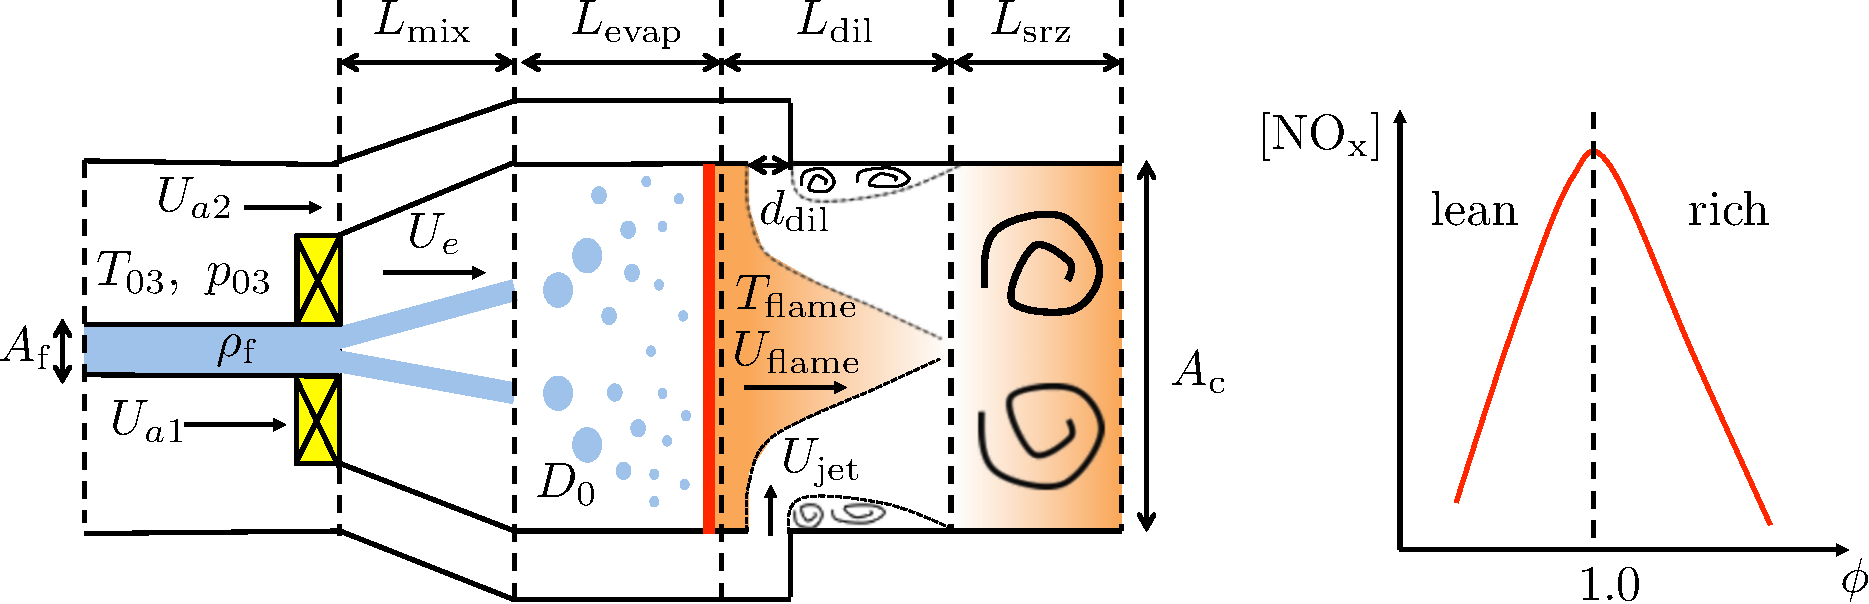
\includegraphics[width=1.0\textwidth]{RQLCombustor.pdf}
		\caption{\label{FIG_RQL} Schematic of a RQL combustor and the effect of equivalence ratio, $\phi$, on combustion.}
	\end{center}
\end{figure}
In an RQL combustor the fuel-air mixture is initially burned rich ($\phi>1$) to limit NO$_\mathrm{x}$ formation through oxygen depletion and the relatively low combustion temperature. However, additional air needs to be injected to minimize other pollutants resultant from the rich burn (e.g., CO). Hence, a secondary mixing process is undergone by injecting air subsequent to the rich zone to yield a lean condition downstream. Similar to rich combustion, the nitric oxide (NO) formation is reduced for lean conditions as shown in the figure.

%=======================================================================================================
\subsection{Combustor Inlet Conditions}
%=======================================================================================================
In this problem, we wish to uncover the inlet conditions of the combustor with respect to the operational conditions. For simplicity, consider this combustor to be a part of an ideal turbojet system. 
\begin{enumerate}
	\item
        Given $T_{04}=1600$ K, $M_0$=0.7, $p_{03}/p_{02}=24$,  $T_0=215$ K, $c_p=1005$ J/kg.K, $P_0=0.146$ bar (43 kft), and the heat of combustion at stoichiometric conditions as evaluated from the previous question, determine the overall fuel-air ratio, $f$, of the combustor.
    \item
    	For n-dodecane, what is the equivalence ratio of the combustor? 
    \item
    	What is the density of the air at the inlet to the combustor, $\rho_{03}$? Use $R=287$ J/kg.K.
\end{enumerate}
%=======================================================================================================
\subsection{Combustor Area}
%=======================================================================================================
For this homework, we will considered a canned combustor geometry. Canned combustors are discrete units with their own casing, fuel injection, liner, and igniter. Other designs include annular and cannular combustors. We will assume for this problem that the combustor geometry is cylindrical and axisymmetric. 

\begin{figure}[!ht!]
	\begin{center}
		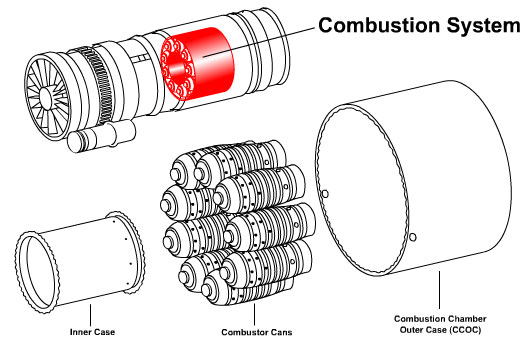
\includegraphics[width=0.9\textwidth]{cannedCombustor.jpg}
		\caption{\label{FIG_CC} Schematic of a canned combustor system}
	\end{center}
\end{figure}

\begin{enumerate}[label=(\alph*)]
	\item
    	Consider a gas-turbine engine with a circular array of canned combustors as shown in the figure. The outer case has specified outer radius, $R_\mathrm{o}$, and inner case radius, $R_\mathrm{i}$. Using this, derive a relation for the maximum number of canned combustors, $n_\mathrm{comb}$, that may fit in the annular section? 
    \item Given $R_\mathrm{o}=0.25$ m and $R_i=0.1$ m, what is the cross-sectional area of each combustor, $A_\mathrm{c}$?
\end{enumerate}
%=======================================================================================================
\subsection{Combustor Length}
%=======================================================================================================
In this problem, we are interested in developing a model that will give the minimum length of the RQL combustor. We will assume that the RQL combustor follows the zonal model shown in Fig.~\ref{FIG_RQL}. The combustor is modeled to be broken up by physical processes into four zones: a evaporation and mixing zone, a flame zone, a dilution zone, and a secondary reaction zone. In reality, there is significant interplay between these regions and the processes can be quite complex, but the goal here is to develop a low-order model, which contains the essential physics of an RQL combustor. 
\begin{enumerate}[label=(\alph*)]
	\item
    	Assume that each physical process has a representative length scale, $L$. Propose a relation, which gives the total length of the combustor. How is the length scale of a process related to its timescale, $\tau$, and its velocity scale, $U$? [Hint: Assume steady-state flow within combustor.]
%=======================================================================================================
    \item \textit{Evaporation and mixing}\\
    	In the injector section of the combustor, liquid fuel is injected with an air co-flow. In this process, we assume turbulence in the flow is strong so that fuel in gas phase mixes with air instantaneously after evaporation forming a rich flammable mixture. With this assumption, the time scale in this process is dominate by evaporation, $\tau_\text{evap}$.
        \begin{enumerate}[label=(\roman*)]
        	\item
            	What is the velocity of the air at the inlet of the combustor, $U_{\mathrm{a}1}$, in terms of $n_\mathrm{comb}$; $\rho_\mathrm{03}$; the ratio of rerouted air to inlet air, $\beta_c=\dot{m}_{a2}/\dot{m}_{a1}$; the total air mass flow rate, $\dot m_\mathrm{a}$ through the core; the combustor area $A_\mathrm{c}$; and the ratio of fuel injection area to the combustor area, $\beta_\mathrm{mix}=A_\mathrm{f}/A_\mathrm{c}$?
            \item
            	Given that the overall fuel-air ratio is $f$, what is the rich fuel-air ratio for the injector section of the combustor, $f_\mathrm{mix}$? What is the equivalence ratio?
        	
            \item 
            The mass evaporation rate of a spherical liquid droplet can be evaluated as 
\begin{equation}
                	\label{EQ_DROPLET}
                	\begin{aligned}
                    	\dot{m}_\mathrm{evap}=2\pi D \frac{\lambda_\mathrm{g}\log(1+\mathcal{B})}{c_{p\mathrm{g}}}
                    \end{aligned}
\end{equation}
where $D$ is the diameter of the droplet, and $\mathcal{B}$ is the Spalding number.
Consider a spherical droplet with initial droplet diameter $D_0$, derive a differential equation that allows you to compute the rate of change of the droplet diameter as a function of the evaporation rate, given in Eq.~\ref{EQ_DROPLET}. Assume that all transport properties are constant, and express $D/D_0$ as a function of time and the evaporation constant  $\beta=8\lambda_\mathrm{g}\log(1+\mathcal{B})/(\rho_\mathrm{f}c_{p\mathrm{g}})$.
        	\item
            	{\it Bonus:} The Rosin-Rammler expression is commonly used to describe the size distribution of droplet diameters and is given by 
                \begin{equation}
                	\label{EQ_RR}
                	\begin{aligned}
                    	F(D_0;D_\sigma,\alpha)=1-\exp\left[\left(\frac{D_0}{D_\sigma}\right)^\alpha\right]
                    \end{aligned}
                \end{equation}
                where $F$ is the total fraction of fuel contained in droplets of diameter less than $D_0$, and $\alpha$ and $D_\sigma$ are parameters of the distribution. Using Eq.~\ref{EQ_RR} and your result from ii, derive an expression for the mean evaporation time for a droplet in the fuel spray. Assume $\alpha=2$.
        	\item
            	Using your results from i and ii, what is the characteristic length of the evaporation section of the combustor, $L_\mathrm{evap}$, in terms of entrainment velocity $U_\mathrm{e}$ and the mean evaporation time $\tau_\mathrm{evap}$? 
        \end{enumerate}
%=======================================================================================================
    \item \textit{Flame}\\
    	Subsequent to the atomization and evaporation section of the combustor, a turbulent flame combusts the rich fuel-air mixture. In this assignment, we will make the coarse assumption that the flame is completely premixed and has negligible length for simplicity (i.e., $L_\mathrm{flame}\approx 0$).  
        \begin{enumerate}[label=(\roman*)]
        	\item
            	What is the fluid speed subsequent to the flame, $U_\mathrm{flame}$, in terms of $U_\mathrm{e}$ and the ratio of adiabatic flame temperature to the unburned reactant temperature, $T_\mathrm{flame}/T_\mathrm{evap}$? Does the speed increase or decrease? Assume isobaric combustion.
            \end{enumerate}
%=======================================================================================================
	\item \textit{Dilution}
		
        The dilution section consists of dilution holes injecting air bypassed from the core flow in a jet-in-crossflow configuration. The holes are arranged azimuthally around the combustor.
         \begin{enumerate}[label=(\roman*)]
         	\item
            	Find a relation for the jet velocity $U_{\mathrm{jet}}$ of each hole in terms of the number of dilution holes ($n_\mathrm{dil}$), the diameter of each hole ($d_\mathrm{dil}$), $\rho_\mathrm{03}$, $\dot m_\mathrm{a}$, and $\beta_\mathrm{c}$. Assume negligible pressure loss during injection.
            \item
            	In the far-field, a jet-in-crossflow displays the self-similar scaling of 
                \begin{equation}
                	\begin{aligned}
                    	c = C_\mathrm{dil}\left(\frac{L}{\xi d_\mathrm{dil}}\right)^{-\frac{2}{3}}
                    \end{aligned}
                \end{equation}
                where $c$ is the concentration in the jet, $C_\mathrm{dil}$ is a constant, $L$ is the distance after injection, and the momentum ratio, $\xi$, is given in terms of the jet and crossflow momentums as
                \begin{equation}
                	\label{EQ_JIC}
                	\begin{aligned}
                	\xi=\sqrt{\frac{\rho_\mathrm{03}U_\mathrm{jet}^2}{\rho_\mathrm{flame}U_\mathrm{flame}^2}}
                    \end{aligned}
                \end{equation}
         
           What is the final concentration $c_\mathrm{f}$ in terms of $\beta_\mathrm{c}$, $f$, and $\dot{m}_a$? [Hint: Consider a mass balance over the dilution zone and find $c_{\rm{f}}$ corresponding to the perfect mixing condition; to simplify your analysis, you can equate $c$ as mass-flow ratio between dilution jets and total mass flow.]
           \item
              Approximate the length of dilution region, $L_\mathrm{dil}$, using the scaling relationship presented in Eq.~\ref{EQ_JIC}.
           \item
           		What is the bulk velocity of the fluid subsequent to the dilution process, $U_\mathrm{dil}$? Assume the mixing is isobaric and adiabatic with both gases having the same specific heats. 
         \end{enumerate}
%=======================================================================================================
    \item \textit{Secondary Reaction Zone}
    
    	The zone subsequent to the jet and cross flow mixing process is assumed to be highly turbulent and without prominent flame structure. In this section of the flow, it is assumed that the relevant timescale of the flow is given by the ignition delay:
        \begin{equation}
          \label{EQ_IGN}
          \begin{aligned}
            \tau_\mathrm{srz}=\frac{A}{p^n\phi^m}\exp\left(\frac{T_\mathrm{a}}{T}\right)
          \end{aligned}
        \end{equation}
        \begin{enumerate}[label=(\roman*)]
        \item
        	Determine $\phi$ in the secondary reaction zone of the combustor assuming half of the fuel was combusted by the flame before the quenching of the dilution jet.
        \item
        	Using Eq.~\ref{EQ_IGN}, find the length of the secondary reaction zone, $L_\mathrm{srz}$. 
        \end{enumerate}
\end{enumerate}
%=======================================================================================================
\section{Model Analysis}
%=======================================================================================================
Following the theoretical analysis, developed so far, we will now extend our engine-design code to implement a combustor module. For this, implement a new function {\tt combustorDesign} that takes as input the engine operating conditions, and outputs combustor geometry. In your combustor design, use the parameters that are provided in Table~\ref{TAB_PARAMS}.

Consider aircraft cruise and take-off conditions (computed in Problem Set \#1) and plot the total length and the zonal lengths of the combustor for $\beta_\mathrm{c}\in[1,10]$.

         \begin{table}[!htb!]
        	\centering
        	\begin{tabular}{|c|c|}\hline
        Parameters & Values \\
        \hline
        $\beta_\mathrm{mix}$ & $100\times 10^{-6}$ \\
        $\dot{m}_\mathrm{a}$ & 1.7 kg/s \\
        $C_\mathrm{s}$ & 0.2  \\
        $\rho_\mathrm{f}$ & 810 kg/m$^3$  \\
        $D_0$ & 50 $\mu$m  \\
        $\beta$ &  0.5$\times 10^{-6}$ m$^2$  \\
        $n_\mathrm{dil}$ &  25 \\
        $d_\mathrm{dil}$ &  1 cm \\
        $C_\mathrm{dil}$ &  0.005 \\
        $T_\mathrm{a}$ &  2100 K \\
        $n$ &  1.0 \\
        $m$ &  0.2 \\
        $A$ &  240 Pa.s \\
        $U_e$ & 0.75 m/s \\
        \hline
        \end{tabular}
          \caption{\label{TAB_PARAMS} Table of the given combustor model parameters.}
          \end{table}

%=======================================================================================================
\bibliographystyle{unsrt}
\bibliography{combustion,shocktube}
%=======================================================================================================
\end{document}
